\documentclass{article}

\usepackage[left=1.5cm, right=1.5cm, top=3cm, bottom = 3cm]{geometry}

\usepackage{amsmath}
\usepackage{amsfonts}
\usepackage{amssymb}
\usepackage{graphicx}
\usepackage{float}
\usepackage{wrapfig}
\usepackage{latexsym}
\usepackage{hyperref}
\usepackage{feynmf}
\linespread{1.1}

\author{SM-at-THU}
\title{\bf{Solutions to Pathria's Statistical Mechanics}\\Chapter 2}

\begin{document}
\maketitle
\section*{Problem 2.1}
The key of the problem is to prove the Jacobian of the transformation equals 1,i.e.
\[D=\frac{\partial (Q_1,\cdots,Q_s,P_1,\cdots,P_s)}{\partial (q_1,\cdots,q_s,p_1,\cdots,p_s)}=1\]
As indicated by $|A B|=|A|/|B^{-1}|$($A$ and $B$ are matrices), we can decompose our transformation into two steps and write
\[D=\frac{\partial (Q_1,\cdots,Q_s,P_1,\cdots,P_s)}{\partial (q_1,\cdots,q_s,P_1,\cdots,P_s)} \bigg/ \frac{\partial (q_1,\cdots,q_s,p_1,\cdots,p_s)}{\partial (q_1,\cdots,q_s,P_1,\cdots,P_s)}\]
If we write $\frac{\partial (Q_1,\cdots,Q_s,P_1,\cdots,P_s)}{\partial (q_1,\cdots,q_s,P_1,\cdots,P_s)}$ explicitly, i.e.
\[ \left| \begin{array}{cc}
 \ \frac{\partial Q_i}{\partial q_j} & \frac{\partial Q_i}{\partial P_j} \\
 0 & \delta^i_j
 \end{array} \right|\]
So,we have
\[\frac{\partial (Q_1,\cdots,Q_s,P_1,\cdots,P_s)}{\partial (q_1,\cdots,q_s,P_1,\cdots,P_s)}=
\left\{ \frac{\partial (Q_1,\cdots,Q_s)}{\partial (q_1,\cdots,q_s)}\right\} _{P=constants}\]

\[D=\left\{ \frac{\partial (Q_1,\cdots,Q_s)}{\partial (q_1,\cdots,q_s)}\right\} _{P=constants} \bigg/
  \left\{ \frac{\partial (p_1,\cdots,p_s)}{\partial (P_1,\cdots,P_s)}\right\} _{q=constants}\]
  
We suppose that the generating function of canonical transformation are $\Phi(q,P,t)$,then we have
\[p_i=\frac{\partial \Phi}{\partial q_i}\]
\[Q_i=\frac{\partial \Phi}{\partial P_i}\]
So,
\[\left\{ \frac{\partial (Q_1,\cdots,Q_s)}{\partial (q_1,\cdots,q_s)}\right\} _{P=constants}= \left| \frac{\partial^2 \Phi}{\partial P_i \partial q_j} \right|\]
\[\left\{ \frac{\partial (p_1,\cdots,P_s)}{\partial (P_1,\cdots,P_s)}\right\} _{P=constants}= \left| \frac{\partial^2 \Phi}{\partial q_i \partial P_j} \right|\]
\\
\[D=\left| \frac{\partial^2 \Phi}{\partial P_i \partial q_j} \right| \bigg/ 
\left| \frac{\partial^2 \Phi}{\partial q_i \partial P_j} \right| =1\]
\section*{Problem 2.2}
\paragraph{(a)}
\[x=r \mathrm{sin} \theta \mathrm{cos}\phi, \ \ y= r \mathrm{sin}\theta \mathrm{sin}\phi, \ \ z=r \mathrm{cos}\theta\]
\[\frac{\partial(x,y,z)}{\partial(r,\theta,\phi)}=r^2 \mathrm{sin}\theta \]
\[\frac{\partial(x,y,z)}{\partial(p_r,p_{\theta},p_{\phi})}=0 \]
\[p_x=p_r \mathrm{sin}\theta \mathrm{cos}\phi + p_{\theta} \frac{\mathrm{cos}\theta \mathrm{cos}\phi}{r}-p_{\phi}\frac{\mathrm{sin}\phi}{r \mathrm{sin}\theta}\]
\[p_y=p_r \mathrm{sin}\theta \mathrm{sin}\phi + p_{\theta} \frac{\mathrm{cos} \theta \mathrm{sin}\phi}{r}+p_{\phi}\frac{\mathrm{cos}\phi}{r \mathrm{sin}\theta}\]
\[p_z=p_r \mathrm{cos}\theta - p_{\theta} \frac{\mathrm{sin}\theta}{r}\]
\[\frac{\partial(p_x,p_y,p_z)}{\partial(p_r,p_{\theta},p_{\phi})}=\frac{1}{r^2 \mathrm{sin}\theta} \]
\[D=\frac{\partial(x,y,z,p_x,p_y,p_z)}{\partial(r,\theta,\phi,p_r,p_{\theta},p_{\phi})}=1 \]
\paragraph{(b)}
\[T=\frac{p_r^2}{2m}+\frac{p_{\theta}^2}{2mr^2}+\frac{p_{\phi}^2}{2mr^2 \mathrm{sin}^2\theta}\]
\begin{eqnarray*}
&\ &\int_{-\infty}^{\infty} dp_{\theta} \int_{-\infty}^{\infty} dp_{\phi} f(r,\theta,\phi,T)\\
&=&2\int_{-\infty}^{\infty} dp_{\theta} \int_{\frac{p_r^2}{2m}+\frac{p_{\theta}^2}{2mr^2}}^{\infty} 
\frac{mr^2 \mathrm{sin}^2\theta dT}{p_{\phi}} f(r,\theta,\phi,T) \\
&=&2mr\mathrm{sin}\theta\int_{-\infty}^{\infty} dp_{\theta} \int_{\frac{p_r^2}{2m}+\frac{p_{\theta}^2}{2mr^2}}^{\infty} \frac{dT}{\sqrt{2mT-p_r^2-\frac{p_{\theta}^2}{r^2}}}f(r,\theta,\phi,T)
\end{eqnarray*}
\section*{Problem 2.3}
The Hamiltonian of the rotator is a function of the angular momentum $L$. 
$$
H = f(L)
$$
Now we divide the phase space into cells with volume $h$ by lines with constant energies:
\begin{figure}[!htp]
\centering
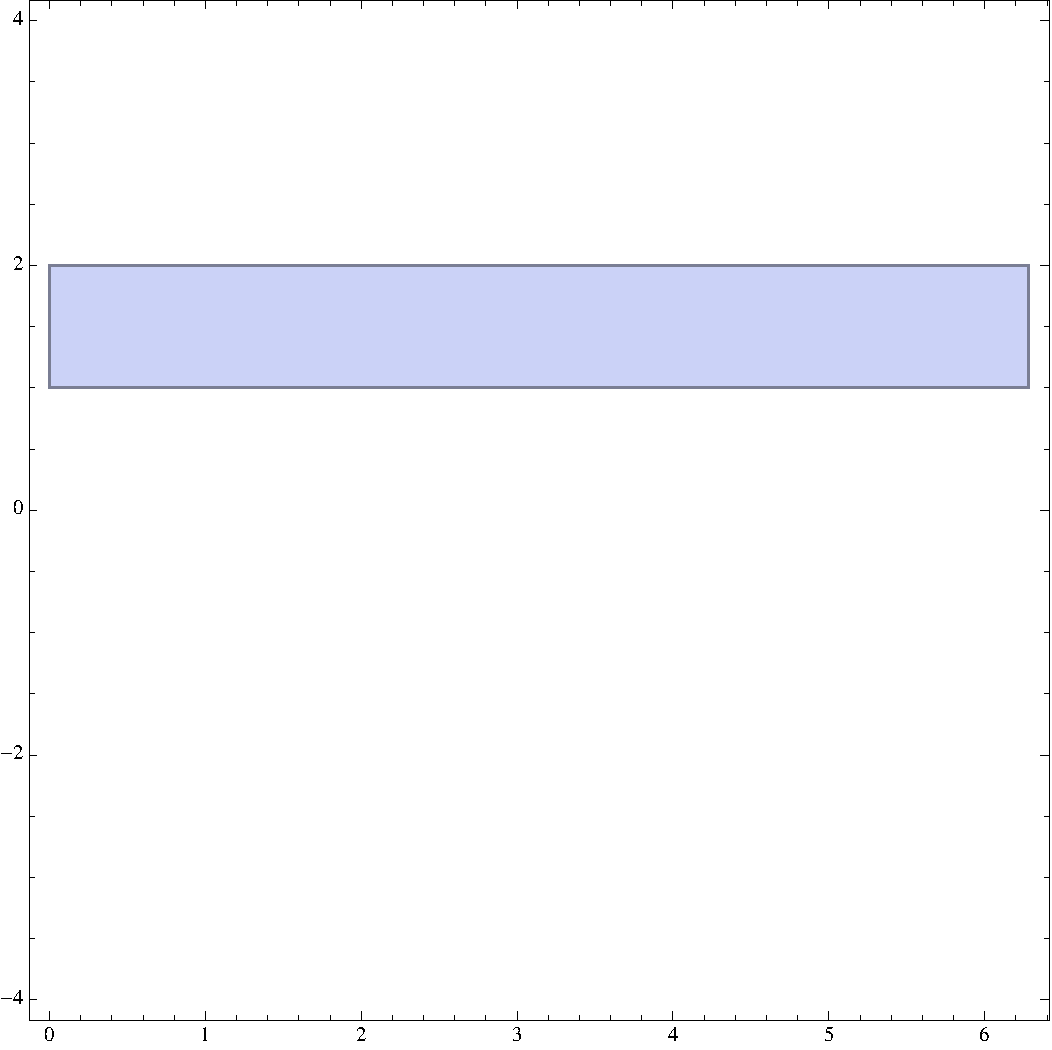
\includegraphics[width=5cm]{./figures/2.3-2.5/pic2.pdf}
\caption{A quantum state in phase space}
\end{figure}\\
Since the angle $\varphi$ varies between $0$ and $2\pi$, angular momentum should be quantized as shown:
$$
h = 2\pi\Delta L\quad \Rightarrow \quad \Delta L =\hbar
$$
Since we starting from the zero line, the eigenvalues of energy should be
\begin{equation}
E_m = f(m\hbar)
\end{equation}
Notice that we get this result by cutting the phase space into slices without solving the Schr$\ddot{\mathrm{o}}$dinger Equation. Because the Hamiltonian commutes with the angular momentum, the eigenenergy is given by eigenvalues of the angular momentum:
$$
-i\hbar \frac{\partial \psi}{\partial\varphi} = L\psi\quad\psi(\varphi) =\psi(\varphi+2\pi)
$$
solve the differential equation and the result is:
$$
L = m\hbar\quad m \in \mathbb{Z}\,.
$$
Now we find that the result we get from the eigenfunction of angular momentum operator is the same as we get from cutting the phase space into cells.


\section*{Problem 2.4}
If we just consider about the orbital angular momentum, it can be written as a function of $p_\theta$ and $p_\varphi$ which are the canonical momentum conjugate to the spherical coordinate variables $\theta$ and $\varphi$: 
\begin{equation}
L^2 = p_\theta^2 + \frac{p_\varphi^2}{\sin^2 \theta}
\end{equation}
thus the phase volume of the region which satisfies $L^2 \leq M^2$ is
\begin{eqnarray}
\bf{\Omega}& = &\int_0^\pi d\theta \int_0^{2\pi} d\varphi \int_{L^2\leq M^2} dp_\theta dp_\varphi\nonumber\\
&=& \int_0^\pi d\theta \int_0^{2\pi} d\varphi \, \pi  M^2\sin\theta\nonumber\\
&=& 4\pi^2 M^2
\end{eqnarray}
Thus the number of microstates is $\Omega = {\bf{\Omega}}/h^2 = M^2/\hbar^2$. Then let us calculate the number by quantized angular momentum. By summing up all the eigenstates of the angular momentum, we get:
\begin{equation}
\Omega = \sum_{j=0}^{j_{\mathrm{max}}}(2j+1) = (j_{\mathrm{max}}+1)^2
\end{equation}
Now we have to determine the number $j_{\mathrm{max}}$. Since we want the absolute value of the angular momentum $ \sqrt{j_{\mathrm{max}}(j_{\mathrm{max}}+1)}\hbar< M$, we can find that $j_{\mathrm{max}}$ is determined by the following equation:
\begin{equation}
j_{\mathrm{max}} = \Big{\lfloor} \frac{\sqrt{1+\frac{4M^2}{\hbar^2}}-1}{2}\Big{\rfloor}
\end{equation}
It is obvious that $j_\mathrm{max} = \lfloor M/\hbar\rfloor -1$ or $j_\mathrm{max} = \lfloor M/\hbar\rfloor$. So the total number of microstates will be:
\begin{equation}
\Omega = \Big{\lfloor} \frac{M}{\hbar}\Big{\rfloor}^2\,\mathrm{or}\,\left(\Big{\lfloor} \frac{M}{\hbar}\Big{\rfloor}+1\right)^2
\end{equation}
If we take the classical limit that $M \gg \hbar$, the result will be:
\begin{equation}
\Omega \simeq \frac{M^2}{\hbar^2}
\end{equation}


\section*{Problem 2.5}
In this problem we need to use the WKB approximation in Quantum Mechanics. 
\begin{figure}[!htp]
\centering
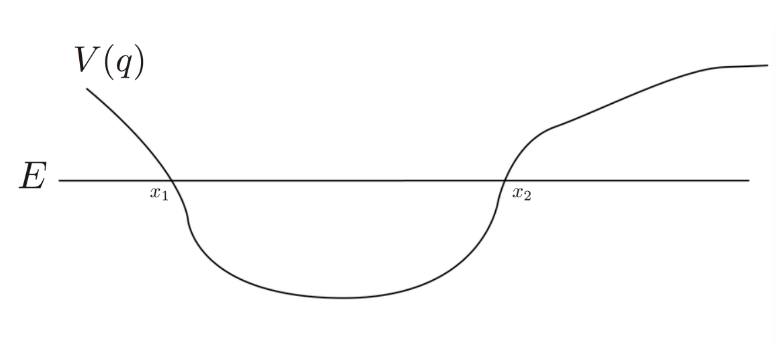
\includegraphics[width=10cm]{./figures/2.3-2.5/pic1.png}
\caption{WKB Approximation}
\end{figure}
In D. Griffiths' book we find that the WKB wave function between two classical turning point $x_1$ and $x_2$ is:
$$
\psi(x) = \frac{2D}{\sqrt{p(x)}}\sin\left[\frac{1}{\hbar}\int_x^{x_2}p(x')dx' + \frac{\pi}{4}\right]\quad\quad x< x_2
$$
or
$$
\psi(x) = -\frac{2D'}{\sqrt{p(x)}}\sin\left[-\frac{1}{\hbar}\int_{x_1}^{x}p(x')dx'-\frac{\pi}{4}\right]\quad\quad x>x_1
$$
in which $p(x) = \sqrt{2m[E-V(x')]}$. We can define:
\begin{eqnarray*}
\theta_1(x) &=& \frac{1}{\hbar}\int_{x_1}^{x}p(x')dx'+\frac{\pi}{4}\\
\theta_2(x) &=& \frac{1}{\hbar}\int_x^{x_2}p(x')dx' + \frac{\pi}{4}
\end{eqnarray*}
Since the two solutions should be the same, the difference between the two $\theta$ functions should be $n\pi, n\in\mathbb{Z}$: 
\begin{equation}
n\pi-\frac{\pi}{2} = \frac{1}{\hbar}\int_{x_1}^{x_2}p(x')dx'
\end{equation}
The integral in classical phase space is
$$
\oint p\,dq = 2 \int_{x_1}^{x_2}p(x')dx'
$$
so finally we can find that 
\begin{equation}
\oint p\,dq = h\left(n-\frac{1}{2}\right)\quad n\in\mathbb{Z}\,.
\end{equation}
\section*{Problem 2.6}
The equation of phase space orbit is:
$$
\frac{1}{2}ml^{2}\dot{\theta}^{2}+\frac{1}{2}mgl\theta^{2}=E
$$
This is a eclipse whose area is:
$$
S=\pi \sqrt{2Eml^{2}}\sqrt{\frac{2E}{mgl}}=2\pi E \sqrt{\frac{l}{g}}=E \tau
$$
\section*{Problem 2.7}
\subparagraph{(i)}
Assume that these N SHOs are distinguishable.To distribute total energy E into such N SHOs,\quad there are 
$$C_{E/\hbar \omega+N/2-1}^{N-1}$$ways. \quad 
Let\quad $E/\hbar \omega >>N$ ,we get the approximate result: 
$$
\frac{1}{(N-1)!} (\frac{E}{\hbar \omega} )^{N-1}
$$
\subparagraph{(ii)}
The total energy of N classical SHOs is:
$$\sum_{i=1}^{N}(\frac{p_i^2}{2m}+\frac{k x_i ^2}{2})=E$$
The phase space volume is:
$$(\frac{2}{\omega})^N E^{N-1} \pi ^N \frac{1}{(N-1)!} dE$$
while dE=$\hbar \omega$,\quad we get\quad $\omega_0=h^N$
\section*{Problem 2.8}
Assume that
\begin{equation}
V_{3N}=\mathop{\int\cdots\int}\limits_{0\le\sum\limits_{i=1}^{N}r_i\le R}\prod_{i=1}^{N}(4\pi r_i^2\mathrm{d}r_i)=C_NR^{3N}
\end{equation}
we can easily see that $C_N$ is a constant. And we have
\begin{equation}
\prod_{i=1}^{N}(4\pi r_i^2\mathrm{d}r_i)=3NC_NR^{3N-1}\mathrm{d}R
\end{equation}
consider the following equation
\begin{eqnarray}
(\int_{0}^{\infty}\mathrm{e}^{-r}r^2\mathrm{d}r)^N&=&\mathop{\int\cdots\int}\limits_{0\le\sum\limits_{i=1}^{N}r_i\le R}\mathrm{e}^{-R}\prod_{i=0}^Nr_i^2\mathrm{d}r_i\\&=&\int_0^\infty\mathrm{e}^{-R}\frac{3NC_N}{(4\pi)^N}R^{3N-1}\mathrm{d}R\\&=&\frac{(3N)!C_N}{(4\pi)^N}
\end{eqnarray}
We also have
\begin{equation}
(\int_{0}^{\infty}\mathrm{e}^{-r}r^2\mathrm{d}r)^N=2^N
\end{equation}
Thus
\begin{equation}
C_N=\frac{(8\pi)^N}{(3N)!}
\end{equation}
and
\begin{equation}
V_{3N}=\mathop{\int\cdots\int}\limits_{0\le\sum\limits_{i=1}^{N}r_i\le R}\prod_{i=1}^{N}(4\pi r_i^2\mathrm{d}r_i)=\frac{(8\pi R^3)^N}{(3N)!}
\end{equation}
The volume of phase space for ralativistic gas $(\varepsilon=pc)$ can be obtained by replacing the $R$ in $V_N$ by $E/c$.
\begin{eqnarray}
V&=&\mathop{\int\cdots\int}\limits_{0\le\sum\limits_{i=1}^{N}r_i\le E/c}4\pi p_i^2\mathrm{d}p_i\\&=&\frac{(8\pi E^3V)^N}{(3N)! c^{3N}}
\end{eqnarray}
The entropy of this system is obtained by 
\begin{equation}
S=k\ln\Omega=k\ln\frac{V}{h^{3N}}
\end{equation}
Using the relations we can get that
\begin{eqnarray}
\frac{\partial S}{\partial E}&=&\frac{1}{T}=\frac{3Nk}{E}\\
\frac{\partial S}{\partial V}&=&\frac{P}{T}=\frac{Nk}{V}\\
C_V&=&(\frac{\partial E}{\partial T})_{N,V}=3Nk\\
C_P&=&\frac{\partial(E+PV)}{\partial T}=4Nk\\
\end{eqnarray}

\section*{Problem 2.9}
Like problem 2.8,
\begin{equation}
\mathop{\int\cdots\int}\limits_{0\le\sum\limits_{i=1}^{3N}|x_i|\le R}(\mathrm{d}x_1\dots\mathrm{d}x_{3N})=C_NR^{3N}
\end{equation}
Thus
\begin{equation}
\mathop{\int\cdots\int}\limits_{0\le\sum\limits_{i=1}^{3N}|x_i|\le R}(\mathrm{e}^{-R}\mathrm{d}x_1\dots\mathrm{d}x_{3N})=\int\mathrm{e}^{-R}C_NR^{3N-1}\mathrm{d}R=C_N(3N)!
\end{equation}
On the other hand,
\begin{equation}
\mathop{\int\cdots\int}\limits_{0\le\sum\limits_{i=1}^{3N}|x_i|\le R}(\mathrm{e}^{-R}\mathrm{d}x_1\dots\mathrm{d}x_{3N})=(\int_{-\infty}^{\infty}\mathrm{d}x_1\dots\mathrm{d}x_{3N})^3N=2^{3N}
\end{equation}
We can see that
\begin{equation}
\mathop{\int\cdots\int}\limits_{0\le\sum\limits_{i=1}^{3N}|x_i|\le R}(\mathrm{d}x_1\dots\mathrm{d}x_{3N})=\frac{(2R)^{3N}}{3N!}
\end{equation}
The phase space for 3N relativistic particles moving in 1 dimension can be obtained using the integral before.
\begin{equation}
V=\frac{(2EL)^{3N}}{(3N)!(c)^{3N}}
\end{equation}
The entropy of this system is obtained by 
\begin{equation}
S=k\ln\Omega=k\ln\frac{V}{h^{3N}}
\end{equation}
Using the relations we can get that
\begin{eqnarray}
\frac{\partial S}{\partial E}&=&\frac{1}{T}=\frac{3Nk}{E}\\
\frac{\partial S}{\partial L}&=&\frac{F}{T}=\frac{3Nk}{L}\\
C_V&=&(\frac{\partial E}{\partial T})_{N,V}=3Nk\\
C_P&=&\frac{\partial(E+FL)}{\partial T}=6Nk\\
\end{eqnarray}

\end{document}
